% !TeX root = RJwrapper.tex
\title{Palmer Archipelago Penguins Data in the palmerpenguins R Package - An
Alternative to Anderson's \emph{Irises}}
\author{by Allison M. Horst, Alison P. Hill, Kristen B. Gorman}

\maketitle

\abstract{%
The famous \emph{Iris} dataset, which exists in the base R
\textbf{datasets} package as \textbf{iris}, is ubiquitous in statistics
and data science education. While the \textbf{iris} measurements were
originally collected by botanist Edgar Anderson, their use in Ronald A.
Fisher's eugenics research has created momentum to address the dataset's
racist use and/or replace \textbf{iris} with alternate data in teaching
materials. Penguin morphological measurements for three species of
\emph{Pygoscelis} penguins that breed on islands throughout the Palmer
Archipelago, Antarctica, provide an approachable, charismatic and near
drop-in replacement for the \textbf{iris} data. Here, we introduce the
\textbf{palmerpenguins} R package and describe the included
\textbf{penguins} data. We directly compare the two datasets for
selected analyses to demonstrate that R users, in particular teachers
and learners currently using the \textbf{iris} data, can switch to the
Palmer Archipelago penguins for many use cases including data wrangling
and visualization, correlation, regression, hypothesis testing,
multivariate analysis (e.g.~PCA), cluster analysis and classification
(e.g.~by k-means).
}

\hypertarget{introduction}{%
\subsection{Introduction}\label{introduction}}

In 1935, American botanist Edgar Anderson measured petal and sepal
structural dimensions (length and width) for 50 flowers from three Iris
species: \emph{Iris setosa}, \emph{Iris versicolor}, and \emph{Iris
virginica} \citep{anderson_irises_1935}. The manageable but non-trivial
size (5 variables and 150 total observations) and characteristics of the
data make it amenable for introducing a wide range of statistical
methods including data wrangling, visualization, regression,
multivariate exploration, and machine learning. Anderson's \emph{Iris}
dataset is built into a number of software packages including the
auto-installed datasets package in R \citep{r_core_team_r_2019},
Python's scikit-learn machine learning library
\citep{pedregosa_scikit-learn_2011}, and the SAS Sashelp library (SAS
Institute, Cary NC), which have facilitated widespread use of the data.
As a result, eighty-five years after the data were initially published,
Anderson's \emph{Iris} measurements are ubiquitous in statistics and
data science course materials and tutorials. \textbf{Sounds great. Why
consider replacing iris?}

In 1936, one year after being described in the Bulletin of the American
Iris Society, Anderson's \emph{Iris} measurements were published in full
by eugenicist and statistician Ronald A. Fisher in \emph{Annals of
Eugenics} \citep{fisher_use_1936}. Regardless of Anderson's initial
motivation, the data today remain inextricably linked to Fisher's
eugenics research and are even commonly, if unfairly, referred to as
``Fisher's iris data.'' For example, an August 2020 search for ``Iris
flower data set'' in Wikipedia returns an article beginning with ``The
iris flower data set or Fisher's iris data\ldots{}'', then later in the
article: ``It is sometimes called Anderson's Iris data set''
\citep{wikipedia_iris_2020}. The \emph{Iris} dataset is similarly
credited to Fisher in statistical computing literature
\citep[\citet{wang_matlab_2015}, \citet{woods_how_2015},
\citet{chen_unsupervised_2018}]{trendafilov_simple_2009}.

There is recent momentum to address Fisher's racist legacy in
statistics. In June 2020, the Committee of Presidents of Statistical
Societies' R.A. Fisher Award and Lectureship was replaced by the
Distinguished Achievement Award and Lectureship, to ``advance a more
just, equitable, diverse, and inclusive statistical community''
\citep{noauthor_institute_2020}. Cambridge University's Gonville and
Caius College recently announced plans to remove a stained-glass window
celebrating Fisher from a campus dining hall \citep{noauthor_sir_2020}.
In the R community, there are calls to (1) address the \emph{Iris}
dataset's use in Fisher's eugenics work, and/or (2) consider using a
different dataset
\citep[\citet{garrick_aden-buie_lets_2020}]{poisot_timothee_its_2020}.
This paper describes (2): a suitable alternative dataset for educators
wanting to replace the \emph{Iris} data in their teaching materials.

Considering \emph{Iris} data usage in data science and statistics
materials, we established the following criteria for a suitable
replacement dataset:

\begin{itemize}
\tightlist
\item
  Available by appropriate license
\item
  Features intuitive subjects and variables understandable to learners
  across fields
\item
  Manageable (but not trivial) in size
\item
  Minimal data cleaning and pre-processing required for most analyses
\item
  Real-world (not manufactured) data
\item
  Similar opportunities for teaching and learning R, data science, and
  statistical skills
\end{itemize}

Here, we describe an alternative to Anderson's \emph{Iris} data that
largely satisfies these criteria: an approachable and charismatic
dataset containing real-world morphological data for three
\emph{Pygoscelis} penguin species that breed throughout the Western
Antarctic Peninsula region, made available through the Long-Term
Ecological Research Network (US LTER). By comparing data structure,
size, and a range of analyses side-by-side for the two datasets, we
demonstrate that the Palmer Archipelago penguin measurements can replace
Anderson's \emph{Iris} data for many use cases in statistics and data
science education.

\hypertarget{data-source}{%
\subsection{Data source}\label{data-source}}

Body size measurements, clutch (i.e., egg laying) observations (e.g.,
date of first egg laid, and clutch completion), and carbon
(\textsuperscript{13}C/\textsuperscript{12}C,
\(\delta\)\textsuperscript{13}C) and nitrogen
(\textsuperscript{15}N/\textsuperscript{14}N,
\(\delta\)\textsuperscript{15}N) stable isotope values of red blood
cells for male and female adult Adélie (\emph{P. adeliae}), chinstrap
(\emph{P. antarcticus}), and gentoo (\emph{P. papua}) penguins on three
islands (Biscoe, Dream and Torgersen) in the Palmer Archipelago were
collected from 2007 - 2009 by Dr.~Kristen Gorman in collaboration with
the \href{https://pal.lternet.edu/}{Palmer Station LTER}, part of the
\href{https://lternet.edu/}{US LTER Network}. For complete data
collection methods and published analyses see Gorman et al.~(2014).

The data in the \textbf{palmerpenguins} R package are available for use
by CC0 license (``No Rights Reserved'') in accordance with the
\href{https://pal.lternet.edu/data/policies}{Palmer Station LTER Data
Policy} and the \href{https://lternet.edu/data-access-policy/}{LTER Data
Access Policy}, and were imported from the
\href{https://environmentaldatainitiative.org/}{Environmental Data
Initiative (EDI) Data Portal} at the links below:

\begin{itemize}
\tightlist
\item
  Adélie penguin data (LTER and Gorman 2020a):
  \href{https://portal.edirepository.org/nis/mapbrowse?packageid=knb-lter-pal.219.5}{KNB-LTER
  Data Package 219.5}
\item
  Chinstrap penguin data (LTER and Gorman 2020b):
  \href{https://portal.edirepository.org/nis/mapbrowse?packageid=knb-lter-pal.221.6}{KNB-LTER
  Data Package 221.5}
\item
  Gentoo penguin data (LTER and Gorman 2020c):
  \href{https://portal.edirepository.org/nis/mapbrowse?packageid=knb-lter-pal.220.5}{KNB-LTER
  Data Package 220.5}
\end{itemize}

\hypertarget{r-package-palmerpenguins}{%
\subsection{\texorpdfstring{R package:
\textbf{palmerpenguins}}{R package: palmerpenguins}}\label{r-package-palmerpenguins}}

R users can install the \textbf{palmerpenguins} package from CRAN by:

\begin{verbatim}
  `install.packages("palmerpenguins")`
\end{verbatim}

Alternatively, the development version of the package can be installed
from GitHub:

\begin{verbatim}
  `remotes::install_github("allisonhorst/palmerpenguins")`
\end{verbatim}

Information, examples, and links to community-contributed materials are
available on the \textbf{palmerpenguins} package website:
\url{https://allisonhorst.github.io/palmerpenguins/}.

The \textbf{palmerpenguins} R package contains two data objects:
\textbf{penguins\_raw} and \textbf{penguins}. The \textbf{penguins\_raw}
data consists of all raw data for 17 variables (Appendix Table 1),
recorded completely or in part for 344 individual penguins, accessed
directly from EDI. As a direct alternative to Anderson's \emph{Iris}
data we recommend using the curated data in \textbf{penguins}, which is
a subset of \textbf{penguins\_raw} retaining all 344 observations,
minimally updated (Appendix B) and reduced to the following eight
variables:

\begin{itemize}
\tightlist
\item
  \emph{species:} a factor denoting the penguin species (Adélie,
  chinstrap, or gentoo)
\item
  \emph{island:} a factor denoting the island (in Palmer Archipelago,
  Antarctica) where observed (Biscoe, Dream or Torgersen)
\item
  \emph{bill\_length\_mm:} a number denoting length of the dorsal ridge
  of a penguin bill (millimeters)
\item
  \emph{bill\_depth\_mm:} a number denoting the depth of a penguin bill
  (millimeters)
\item
  \emph{flipper\_length\_mm:} an integer denoting the length of a
  penguin flipper (millimeters)
\item
  \emph{body\_mass\_g:} an integer denoting the weight of a penguin's
  body (grams)
\item
  \emph{sex:} a factor denoting the sex of a penguin sex (male, female)
  based on molecular data
\item
  \emph{year:} an integer denoting the year of study (2007, 2008 or
  2009)
\end{itemize}

The same data exist as comma-separated value (CSV) files in the package
(``penguins\_raw.csv'' and ``penguins.csv''), and can be read in using
the built-in \texttt{path\_to\_file()} function in
\textbf{palmerpenguins}. For example,

\begin{verbatim}
    library(tidyverse)
    library(palmerpenguins)
    df <- read_csv(path_to_file(“penguins.csv”))
\end{verbatim}

will read in ``penguins.csv'' as if from an external file, thus
automatically parsing \emph{species}, \emph{island} and \emph{sex}
variables as characters. This option allows users opportunities to
practice or demonstrate reading in data from a CSV, then updating
variable class (e.g.~characters to factors).

\hypertarget{other-data-access-options}{%
\subsection{Other data access options}\label{other-data-access-options}}

Python: Python users can access the penguins data in the
\textbf{seaborn} data visualization library (Waskom et al.~2017).
Example code to load the data in Python:

\begin{verbatim}
    import seaborn as sns
    df = sns.load_dataset('penguins') 
\end{verbatim}

Julia: Julia users can access the penguins data in the
\textbf{PalmerPenguins.jl} package. Example code to import the penguins
data through \textbf{PalmerPenguins.jl}:

\begin{verbatim}
    julia> using DataFrames
    julia> df = DataFrame(table)
\end{verbatim}

\hypertarget{software-and-code}{%
\subsection{Software and code}\label{software-and-code}}

All analyses were performed in the R language environment using version
3.6.2 (R Core Team 2019). Complete code for this paper is shared in the
Supplemental Material. We acknowledge the following R packages used in
analyses, with gratitude to developers and contributors:

\begin{itemize}
\tightlist
\item
  \textbf{tidyverse} (Wickham et al.~2019), for data import and cleaning
\item
  \textbf{ggplot2} (Wickham 2016:2), for data visualizations
\item
  \textbf{here} (Müller 2017), for file path control
\item
  \textbf{kableExtra} (Zhu 2019) for finalized tables
\item
  \textbf{gt} (Iannone, Cheng, and Schloerke 2020) for finalized tables
\item
  \textbf{GGally} (Schloerke et al.~2020), for pairs plots
\item
  \textbf{patchwork} (Pedersen 2019), for compound figures
\item
  \textbf{shadowtext} (Yu 2019), to add a background color to text
  labels
\item
  \textbf{recipes} (Kuhn and Wickham 2020), for data pre-processing
\item
  \textbf{base} and \textbf{stats} (R Core Team 2019) for various
  analyses throughout
\item
  \textbf{pkgdown} (ref) was used to build the package website
\end{itemize}

\hypertarget{selected-comparisons-between-iris-and-penguins}{%
\subsection{\texorpdfstring{Selected comparisons between \textbf{iris}
and
\textbf{penguins}}{Selected comparisons between iris and penguins}}\label{selected-comparisons-between-iris-and-penguins}}

The \textbf{penguins} data in \textbf{palmerpenguins} is generally
useful and approachable for data science and statistics education, and
is uniquely well-suited to replace the \textbf{iris} dataset.
Comparisons presented are selected examples for common \textbf{iris}
uses, and are not exhaustive.

\hypertarget{data-structure-and-sample-size}{%
\subsubsection{Data structure and sample
size}\label{data-structure-and-sample-size}}

Both \textbf{iris} and \textbf{penguins} are in tidy format {[}ref{]}
with each column denoting a single variable and each row containing
measurements for a single \emph{Iris} flower or penguin. The two
datasets are comparable in size: dimensions (columns × rows) are 5 × 150
and 8 × 344 for \textbf{iris} and \textbf{penguins}, respectively, and
sample sizes within species are similar (Table 1). Notably, sample sizes
differ for the three penguin species, while sample sizes in
\textbf{iris} are equal (n = 50 for each Iris species). Multiple factor
variables in \textbf{penguins} (\emph{species}, \emph{island} and
\emph{sex}) along with \emph{year} create additional opportunities for
grouping, compared to the single factor (\emph{species}) in
\textbf{iris}.

Unlike \textbf{iris}, which contains only complete cases, the
\textbf{penguins} dataset contains a small number of missing values
(n\textsubscript{missing} = 19, out of 2,752 total values). Missing
values and unequal sample sizes are common in real-world data, and we
believe add learning value to \textbf{penguins}.

\begin{Schunk}
\begin{table}

\caption{\label{tab:unnamed-chunk-1}Grouped sample size for iris (by species; n = 150 total) and penguins (by species and sex; n = 344 total). Penguins can be further grouped by variables for island and study year.}
\centering
\begin{tabular}[t]{l|c|l|c|c|c}
\hline
\multicolumn{2}{c|}{Iris sample size (by species)} & \multicolumn{4}{c}{Penguin sample size (by species and sex)} \\
\cline{1-2} \cline{3-6}
Iris species & Sample size & Penguin species & Female & Male & NA\\
\hline
setosa & 50 & Adélie & 73 & 73 & 6\\
\hline
versicolor & 50 & chinstrap & 34 & 34 & 0\\
\hline
virginica & 50 & gentoo & 58 & 61 & 5\\
\hline
\end{tabular}
\end{table}

\end{Schunk}

\hypertarget{continuous-quantitative-variables}{%
\subsubsection{Continuous quantitative
variables}\label{continuous-quantitative-variables}}

Distributions, relationships between variables and clustering can be
visually explored between species for the four structural size
measurements in \textbf{penguins} (flipper length, body mass, bill
length and depth; Figure \ref{fig:penguins-pairs}) and \textbf{iris}
(sepal width and length, petal width and length; Figure
\ref{fig:iris-pairs}).

\begin{Schunk}
\begin{figure}
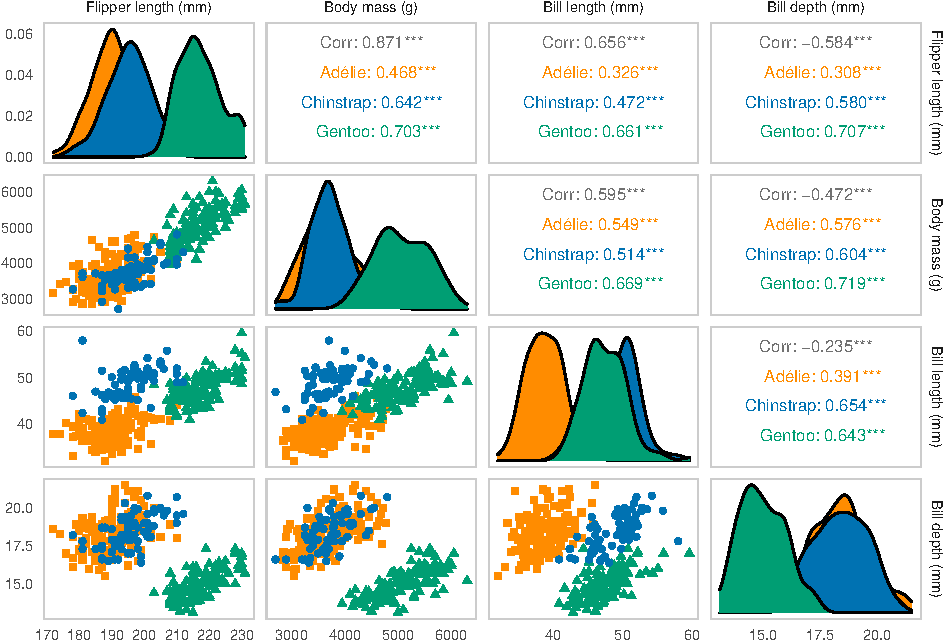
\includegraphics{penguins_files/figure-latex/penguins-pairs-1} \caption[Distribution and correlations for numeric variables in the penguins data (flipper length (mm), body mass, (g) bill length (mm) and bill depth (mm)) for the three observed species]{Distribution and correlations for numeric variables in the penguins data (flipper length (mm), body mass, (g) bill length (mm) and bill depth (mm)) for the three observed species: gentoo (green, triangles); chinstrap (blue, circles); and Adélie (orange, squares). Correlations are Pearson's r (*p < 0.05; **p < 0.01; ***p < 0.001).}\label{fig:penguins-pairs}
\end{figure}
\end{Schunk}

\begin{Schunk}
\begin{figure}
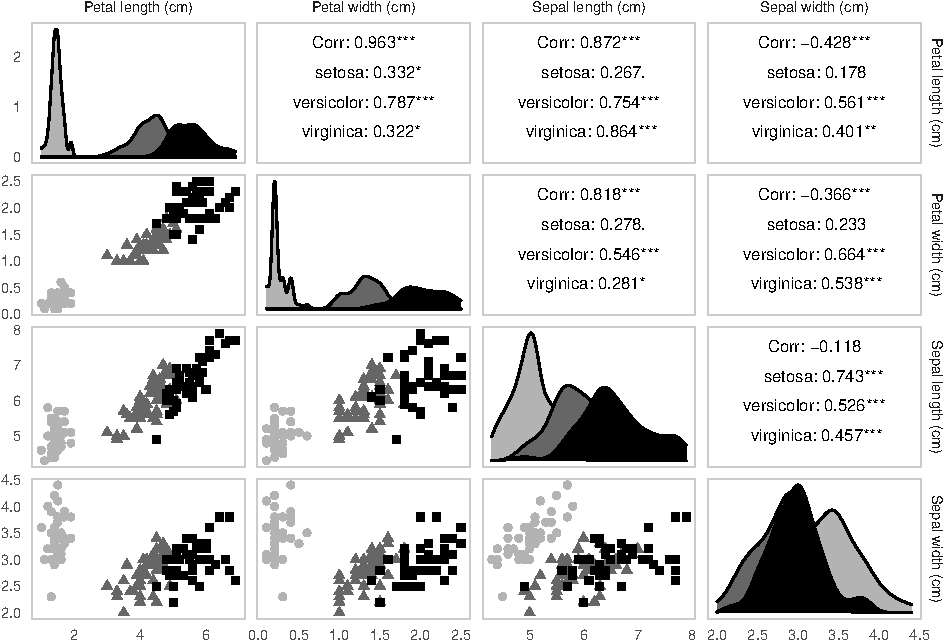
\includegraphics{penguins_files/figure-latex/iris-pairs-1} \caption[Distribution and correlations for numeric variables in the iris data (petal length (cm), petal width (cm), sepal length (cm) and sepal width (cm)) for the three included Iris species]{Distribution and correlations for numeric variables in the iris data (petal length (cm), petal width (cm), sepal length (cm) and sepal width (cm)) for the three included Iris species: setosa (light gray, circles); versicolor (dark gray, triangles); and virginica (black, squares). Correlations are Pearson's r (*p < 0.05; **p < 0.01; ***p < 0.001).}\label{fig:iris-pairs}
\end{figure}
\end{Schunk}

There exist numerous opportunities to explore linear relationships and
correlations in \textbf{penguins} and \textbf{iris} both within and
across species (Figures \ref{fig:penguins-pairs} \&
\ref{fig:iris-pairs}). Here, we highlight one comparison that is
uniquely similar: petal dimensions (petal length versus petal width)
from \textbf{iris}, and penguin size (flipper length versus body mass)
in \textbf{penguins} (\ref{fig:linear-example}). The overall trend
across all three species is approximately linear for both \textbf{iris}
and \textbf{penguins}. Teachers may encourage students to explore how
simple linear regression results and predictions differ when the species
variable is omitted, compared to multiple linear regression with species
included (\ref{fig:linear-example}).

\begin{Schunk}
\begin{figure}[htbp]

{\centering 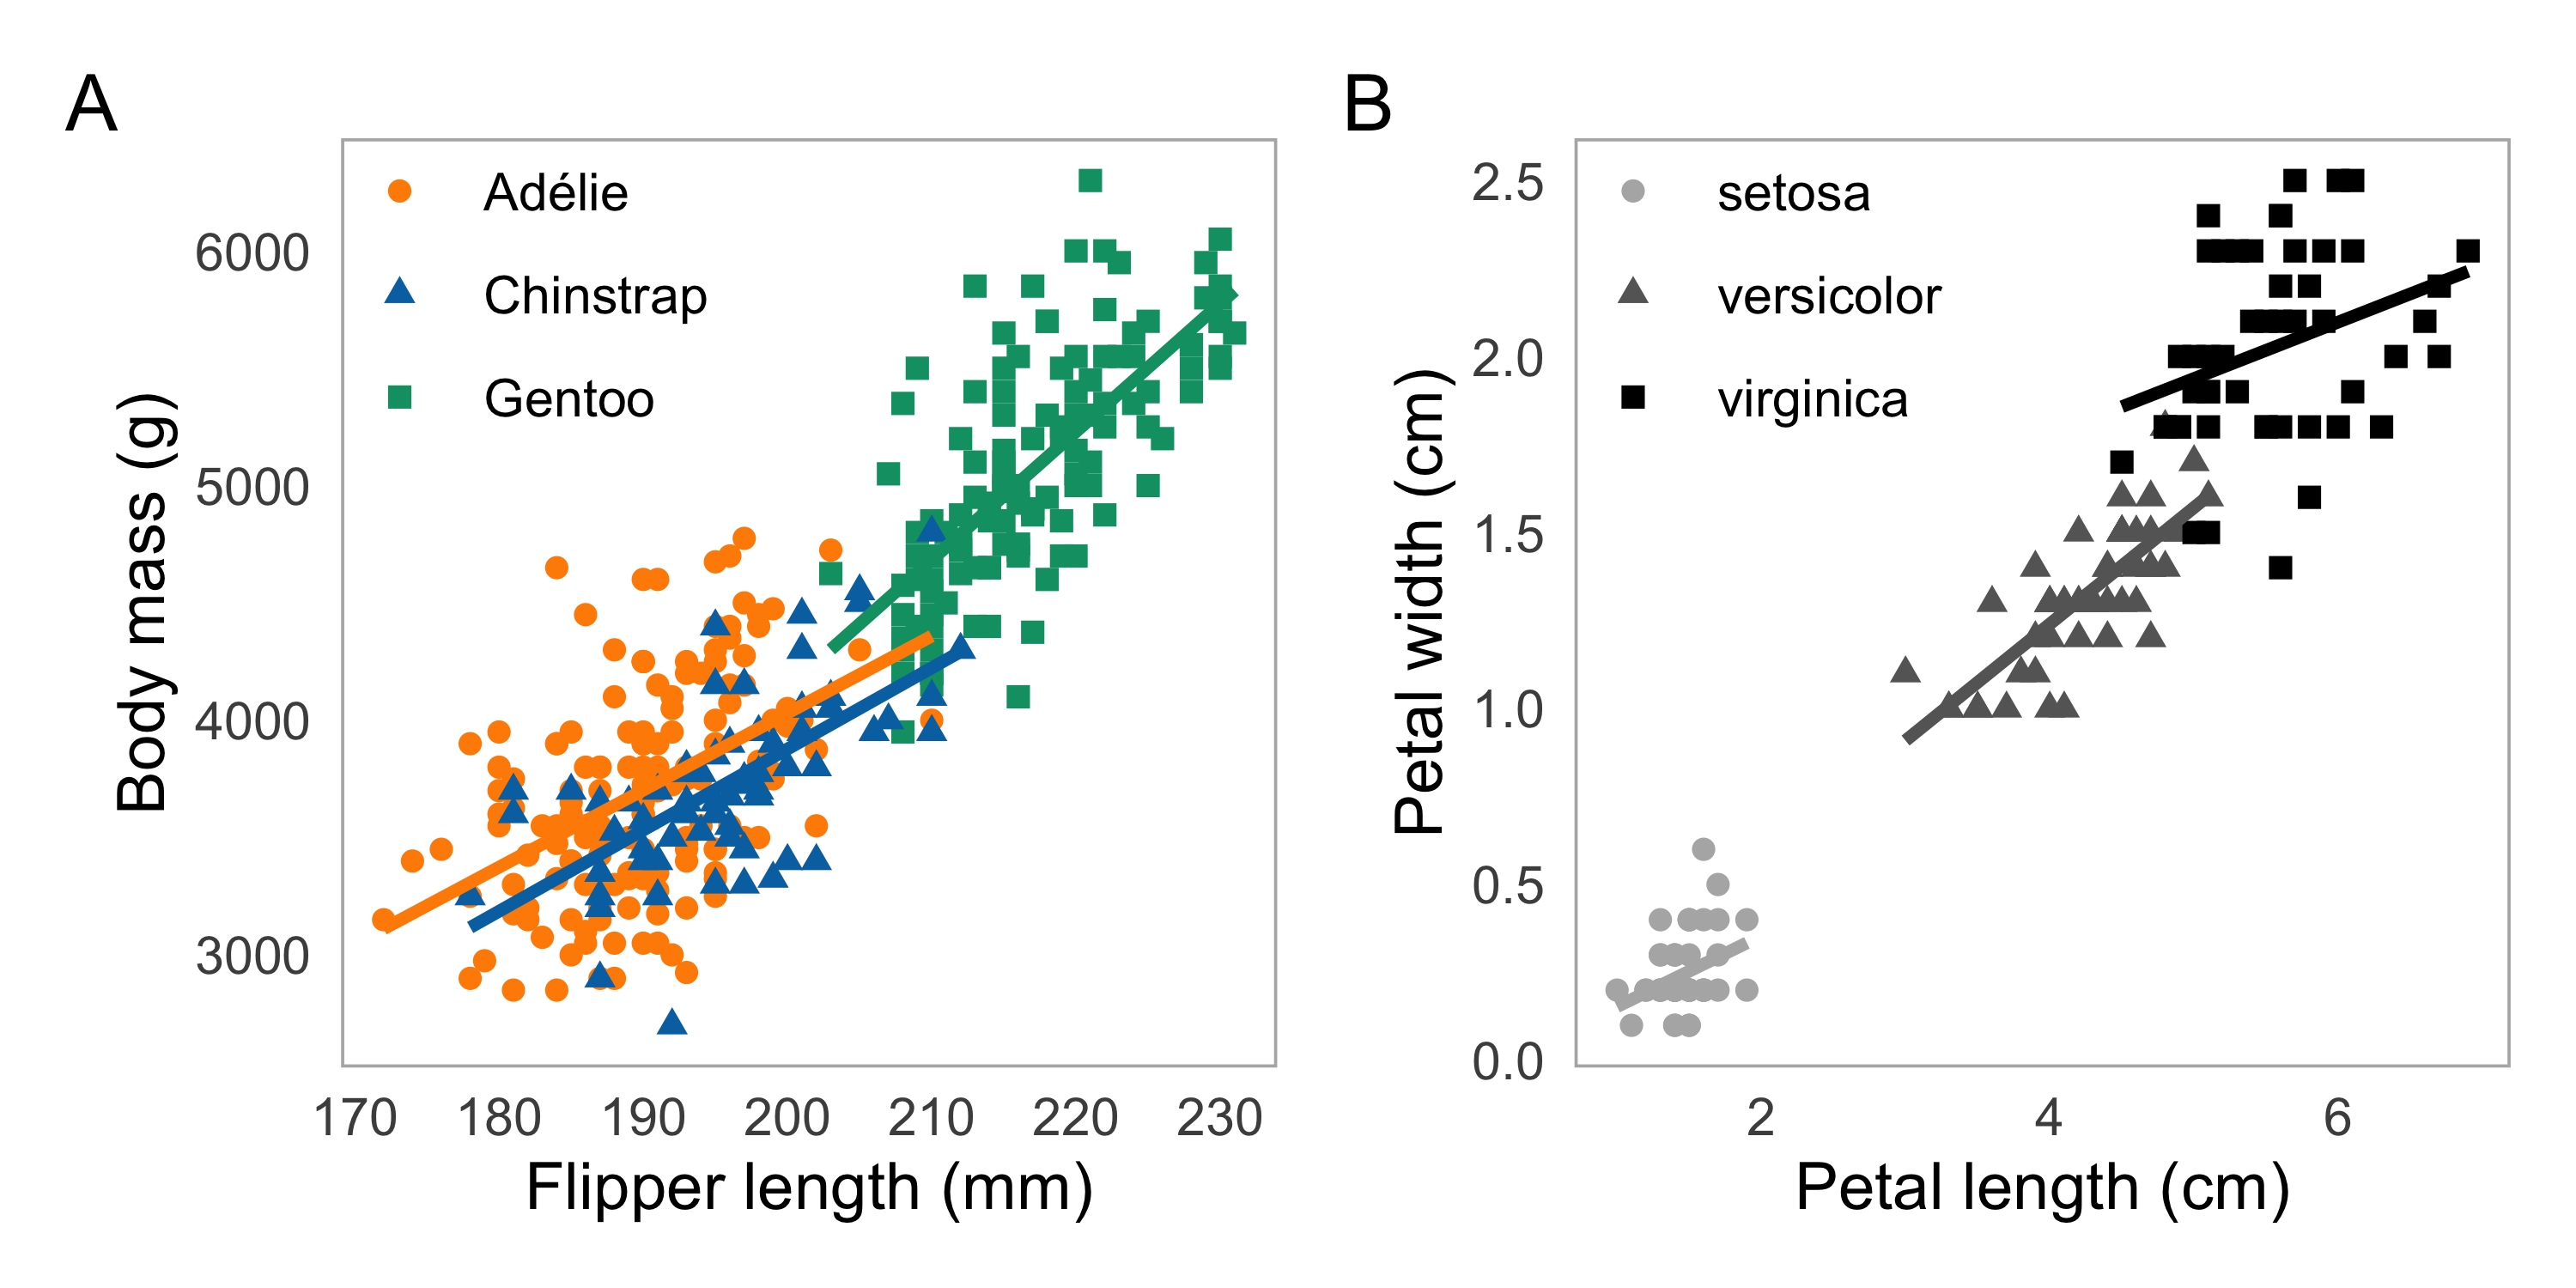
\includegraphics[width=6in]{fig/linear_example} 

}

\caption[Representative linear relationships for penguin flipper length (mm) and body mass (g) for Adélie (orange circles), chinstrap (blue triangles), and gentoo (green squares) penguins (A), and iris petal length (cm) and width (cm) for setosa (light gray circles), versicolor (dark gray triangles) and virginica (black squares) irises (B)]{Representative linear relationships for penguin flipper length (mm) and body mass (g) for Adélie (orange circles), chinstrap (blue triangles), and gentoo (green squares) penguins (A), and iris petal length (cm) and width (cm) for setosa (light gray circles), versicolor (dark gray triangles) and virginica (black squares) irises (B). Within-species linear model is visualized for each penguin or iris species.}\label{fig:linear-example}
\end{figure}
\end{Schunk}

Notably, distinctions between species are clearer for iris petals -
particularly, the much smaller petals for \emph{Iris setosa} - compared
to penguins, in which Adélie and chinstrap penguins are largely
overlapping in body size (body mass and flipper length), and are both
generally smaller than gentoos.

Simpson's Paradox is a data phenomenon in which a trend observed between
variables is reversed when data are pooled, omitting a meaningful
variable. While often taught and discussed in statistics courses,
finding a real-world and approachable example of Simpson's paradox can
be a challenge. Here, we show one (of several possible; see Figure
\ref{fig:penguins-pairs}) Simpson's Paradox examples in
\textbf{penguins}: exploring bill dimensions with and without
\emph{species} included (Figure \ref{fig:simpsons}). When penguin
\emph{species} is omitted (Figure \ref{fig:simpsons} A), bill length and
depth appear negatively correlated overall. The trend is reversed when
\emph{species} is included, revealing an obviously positive correlation
between bill length and bill depth within species (Figure
\ref{fig:simpsons} B).

\begin{Schunk}
\begin{figure}[htbp]

{\centering 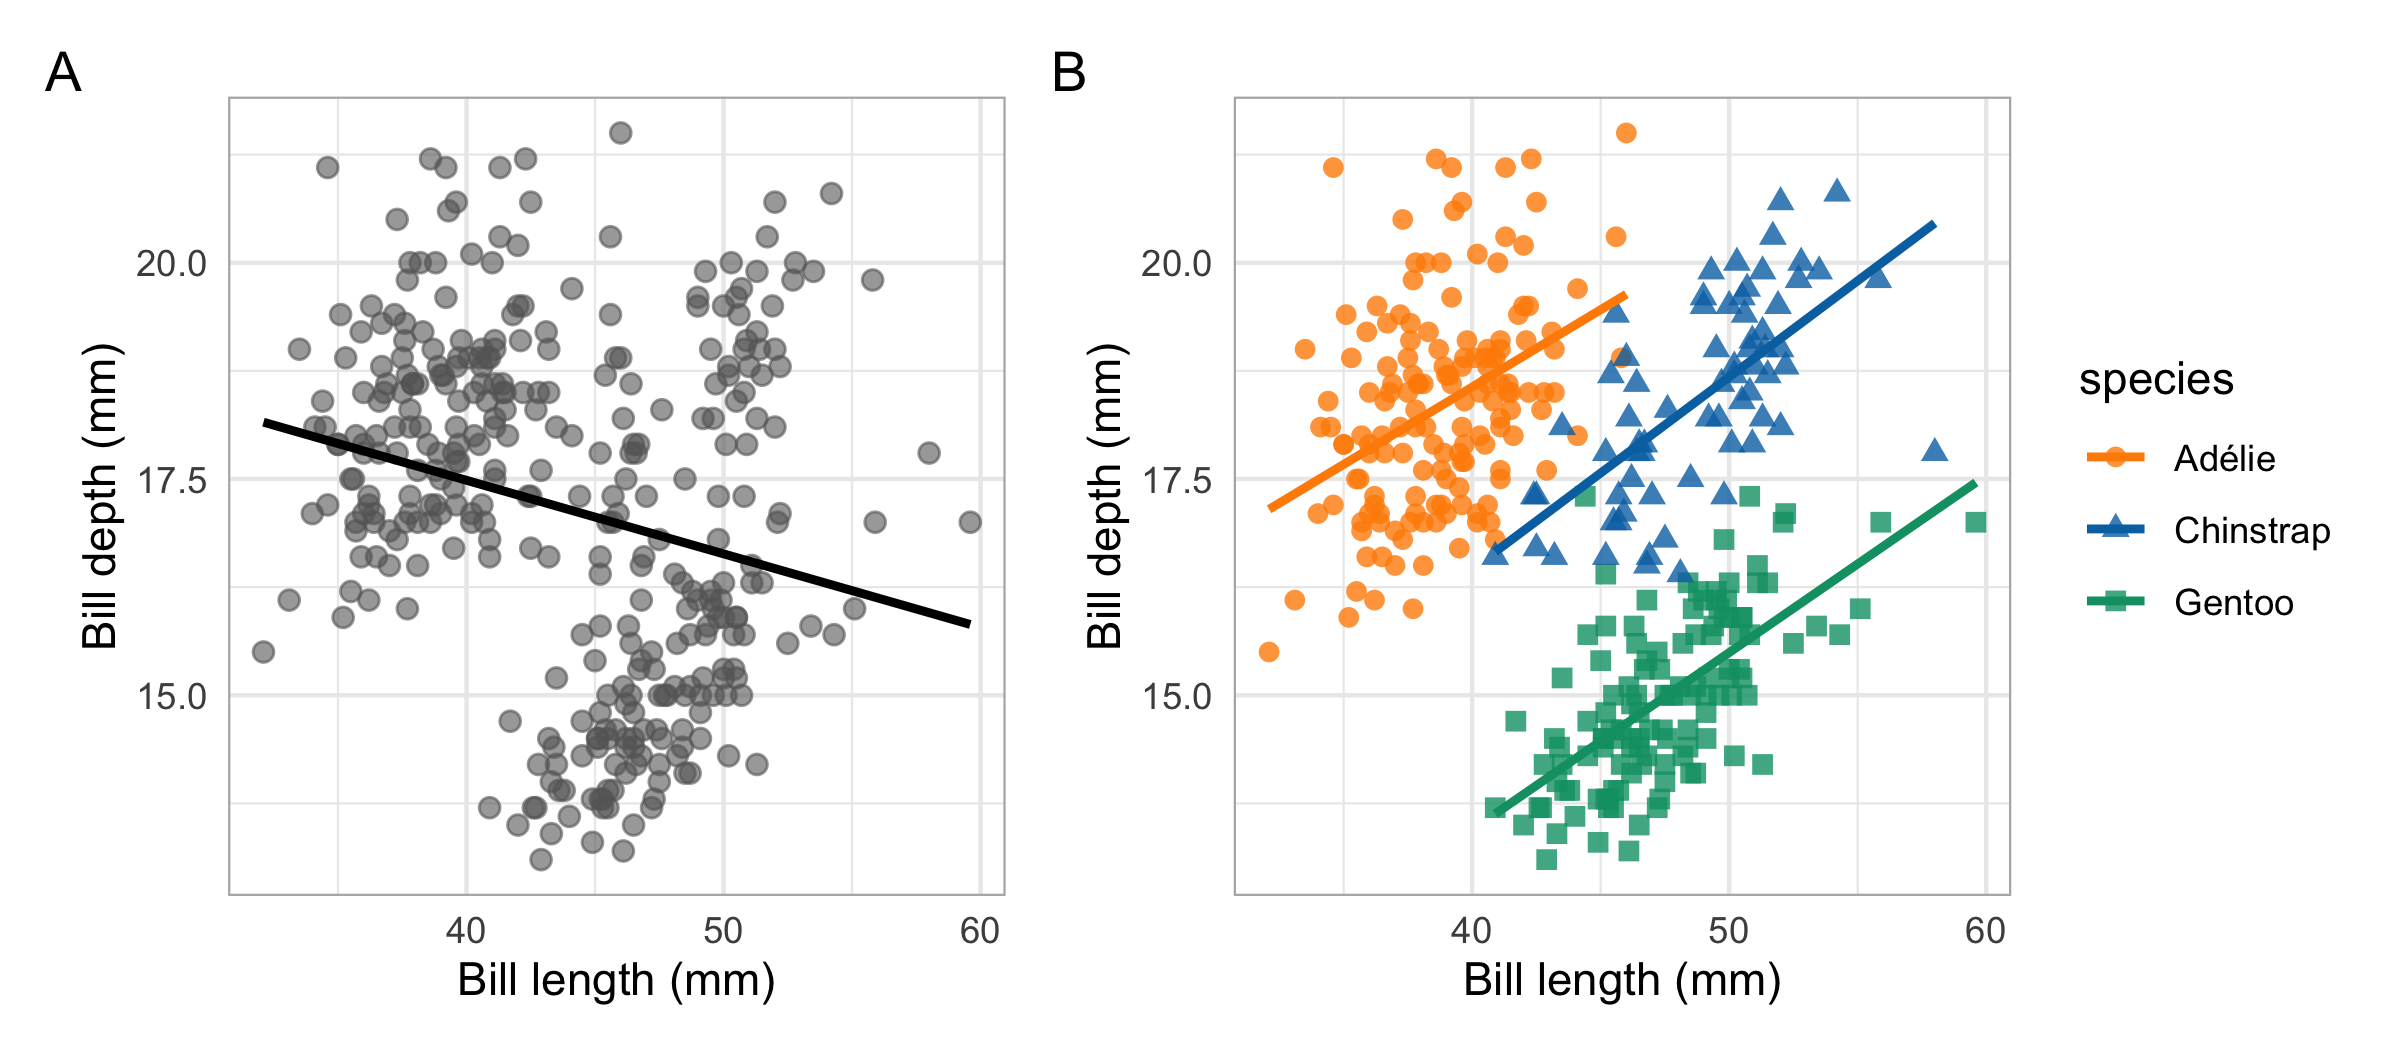
\includegraphics[width=6in]{fig/simpson_gg} 

}

\caption[Trends for penguin bill dimensions (bill length and bill depth, millimeters) if the ‘species’ variable is excluded (A) or included (B), illustrating Simpson’s Paradox]{Trends for penguin bill dimensions (bill length and bill depth, millimeters) if the ‘species’ variable is excluded (A) or included (B), illustrating Simpson’s Paradox. Note: linear regression for bill dimensions without including species in (A) is ill-advised; the linear trendline is only included to visualize trend reversal for Simpson’s Paradox when compared to (B).}\label{fig:simpsons}
\end{figure}
\end{Schunk}

\hypertarget{principal-component-analysis}{%
\subsubsection{Principal component
analysis}\label{principal-component-analysis}}

Principal component analysis (PCA) is a dimensional reduction method
commonly used to explore patterns in multivariate data. PCA tutorials
frequently employ the \textbf{iris} dataset, which is useful for
teaching the method due to multivariate normality, and clear,
approachable outcomes for variable loadings and clustering.

A comparison of PCA with the four variables of structural size
measurements in \textbf{penguins} and \textbf{iris} (both normalized
prior to PCA) reveals highly similar results (Figure \ref{fig:pca}). For
both datasets, one species is distinct (gentoo penguins, and setosa
irises) while the other two species (chinstrap/Adélie and
versicolor/virginica) appear somewhat overlapping in the first two
principal components (Figure \ref{fig:pca} A,B). Variance explained by
each principal component (PC) is similar, particularly for PC1 and PC2:
for \textbf{penguins}, 88.15\% of total variance is captured by the
first two PCs, compared to 95.81\% for \textbf{iris}, with a similarly
large percentage of variance captured by PC1 and PC2 in each (Figure
\ref{fig:pca} C,D).

\begin{Schunk}
\begin{figure}[htbp]

{\centering 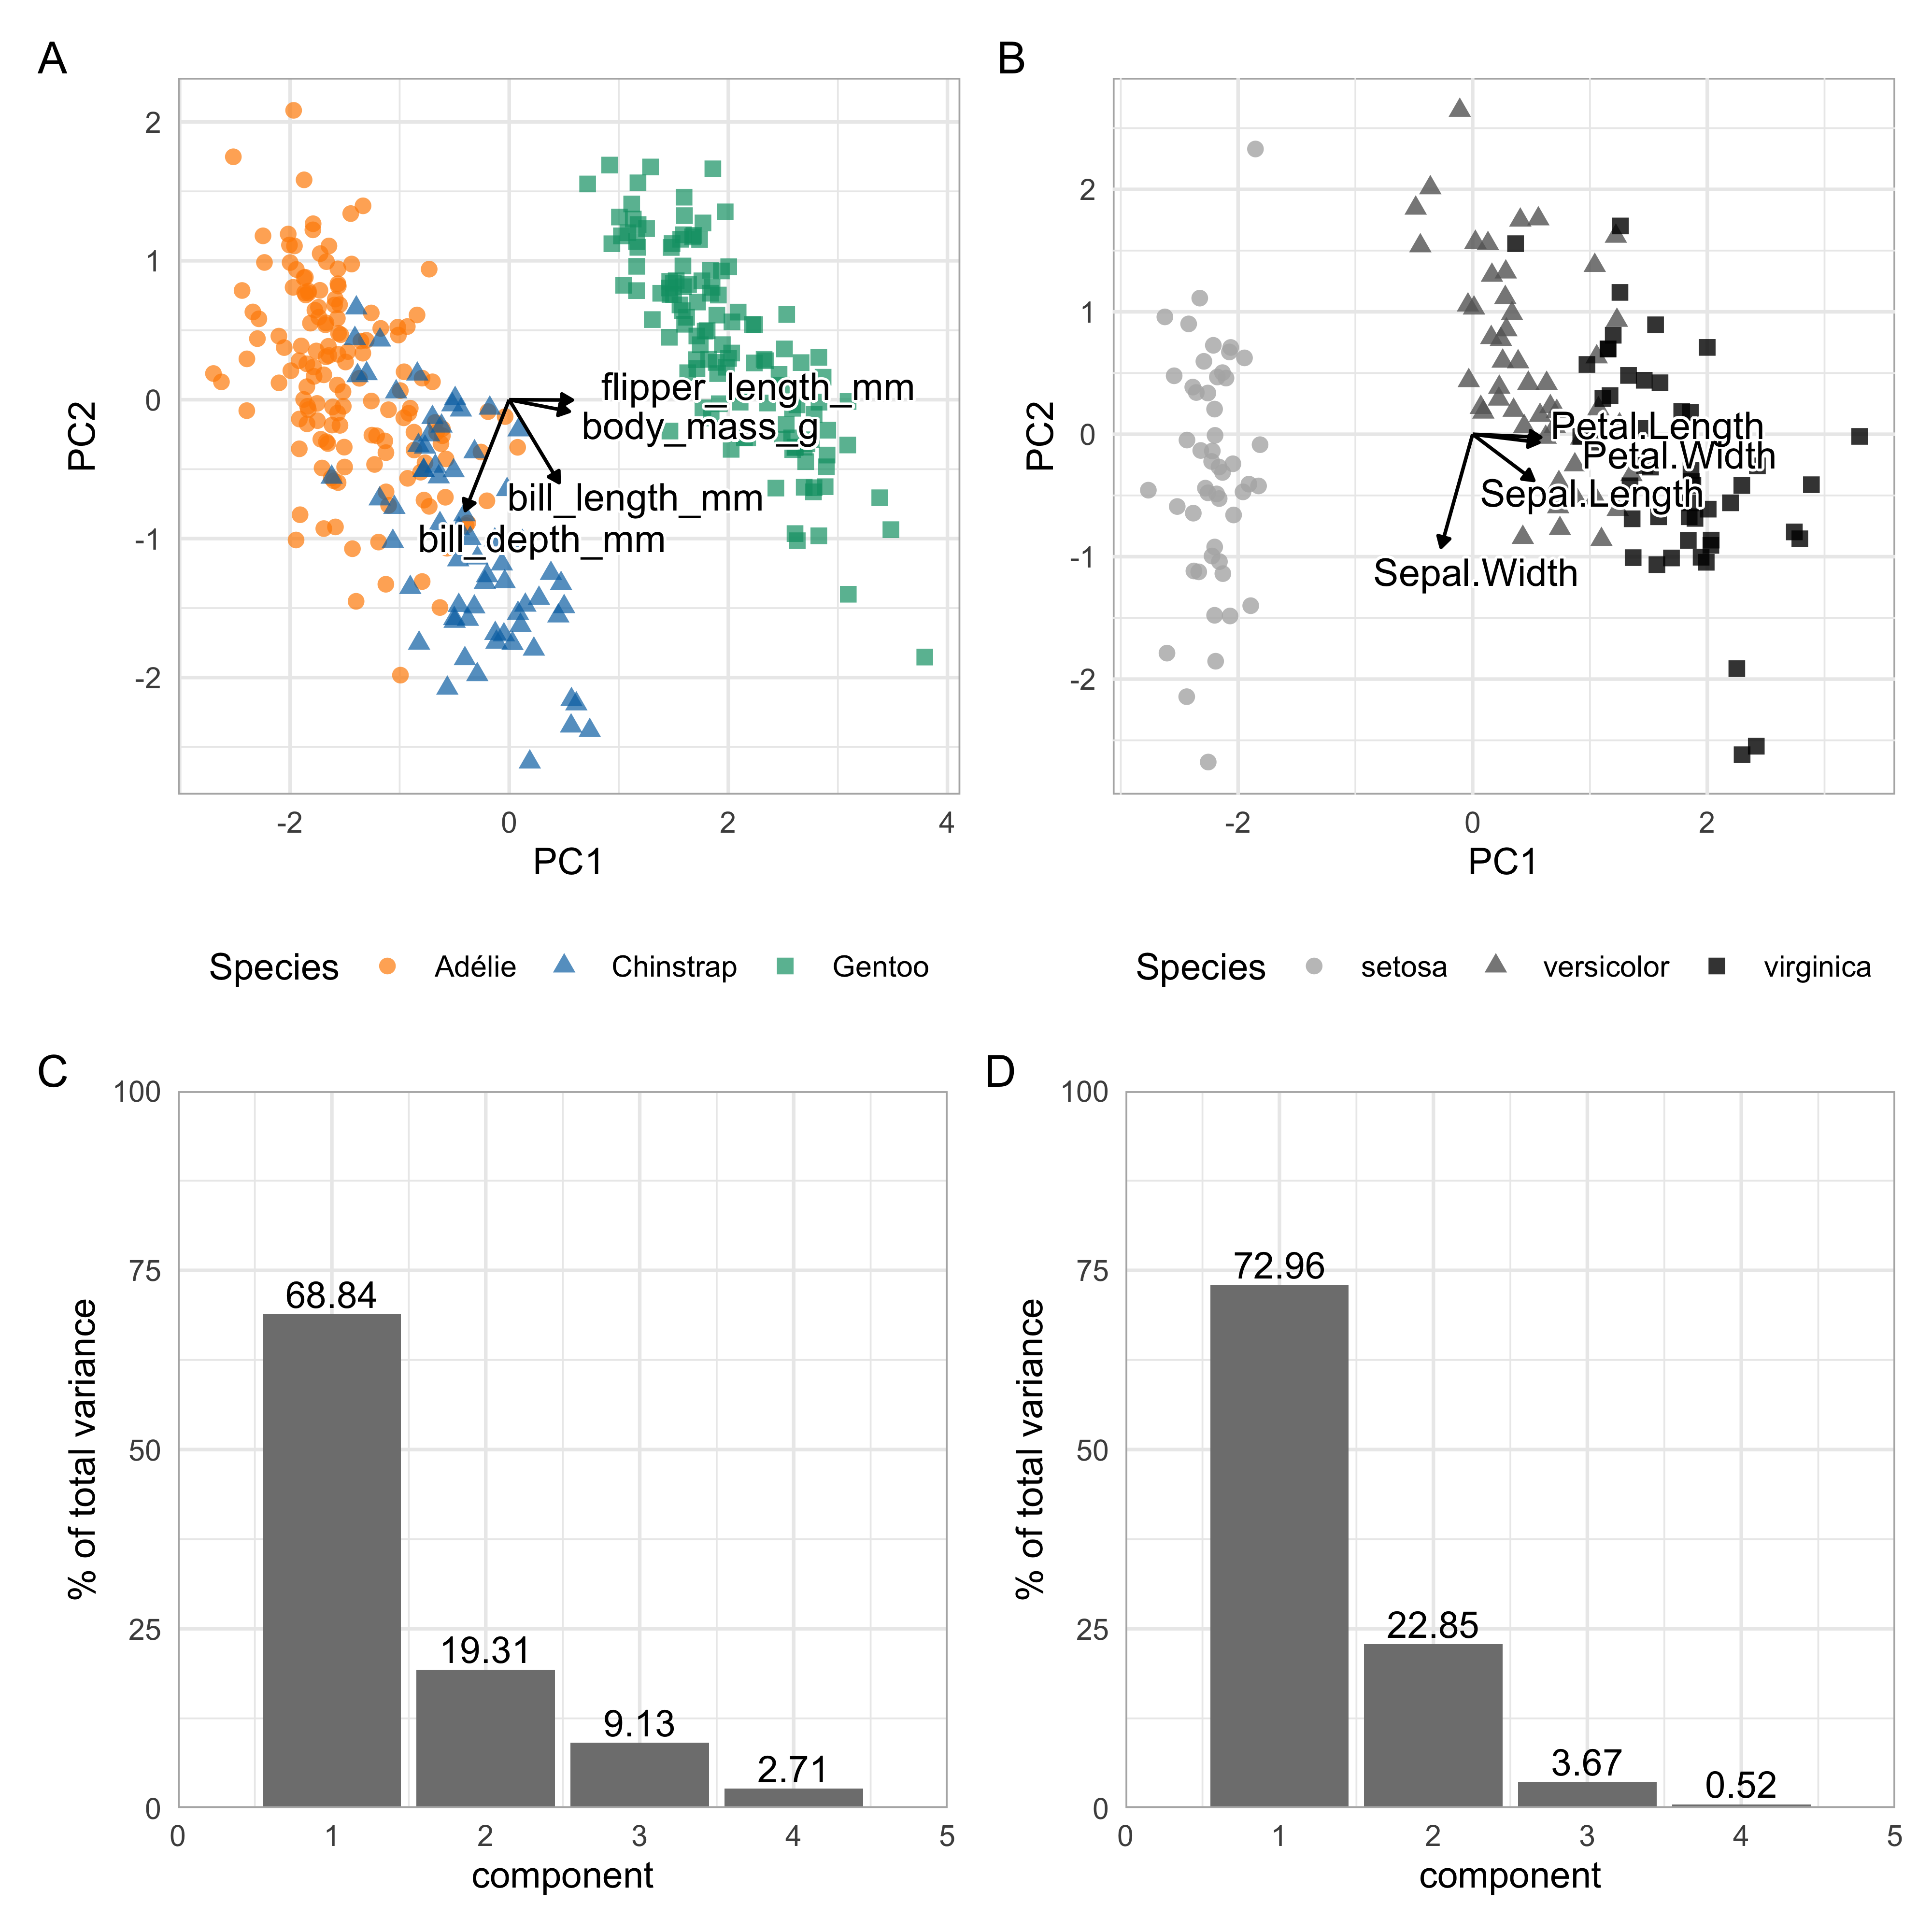
\includegraphics[width=6in]{fig/pca_plots} 

}

\caption[Principal component analysis biplots and scree plots for structural size measurements in penguins (A,C) and iris (B,D), revealing similarities in multivariate patterns, variable loadings, and variance explained by each component]{Principal component analysis biplots and scree plots for structural size measurements in penguins (A,C) and iris (B,D), revealing similarities in multivariate patterns, variable loadings, and variance explained by each component. For penguins, variables are flipper length (mm), body mass (g), bill length (mm) and bill depth (mm); groups are visualized by species (Adélie = orange circles, chinstrap = blue triangles, gentoo = green squares). For iris, variables are petal length (cm), petal width (cm), sepal length (cm) and sepal width (cm); groups are visualized by species (setosa = light gray circles, versicolor = dark gray triangles, virginica = black squares). Values above scree plot columns (C,D) indicate percent of total variance explained by each of the four principal components.}\label{fig:pca}
\end{figure}
\end{Schunk}

\hypertarget{k-means-clustering}{%
\subsubsection{K-means clustering}\label{k-means-clustering}}

Unsupervised clustering by k-means is a common and popular entryway to
machine learning and classification, and frequently employs the
\textbf{iris} data for introductory examples. The \textbf{penguins} data
provides similar opportunities for introducing k-means clustering. For
simplicity, we compare k-means clustering using only two variables for
each dataset: for \textbf{iris}, petal width and petal length, and for
\textbf{penguins}, bill length and bill depth. All variables are scaled
prior to k-means. Three clusters (\emph{k} = 3) are specified for each
since there are three species of both \emph{Iris} (\emph{setosa},
\emph{versicolor}, and \emph{virginica}) and penguins (Adélie, chinstrap
and gentoo).

K-means clustering with penguin bill dimensions and iris petal
dimensions yields largely distinct clusters each dominated by one
species (\ref{fig:kmeans}). For iris petal dimensions, k-means yields a
perfectly separated cluster (Cluster 1) containing all 50 setosa iris
observations and zero misclassified virginica or versicolor irises
(Table 2). While clustering is not perfectly distinct for any penguin
species, each species is largely contained within a single cluster, with
little overlap from the other two species. For example, considering
Adélie penguins (orange observations in Figure \ref{fig:kmeans} A): 147
(out of 151) Adélie penguins are assigned to Cluster 1, zero are
assigned to Cluster 2, and 4 are assigned to the chinstrap-dominated
Cluster 3 (Table 2). Only 5 (of 68) chinstrap penguins and 1 (of 123)
gentoo penguins are assigned to the Adélie-dominated Cluster 1 (Table
2).

\begin{Schunk}
\begin{figure}[htbp]

{\centering 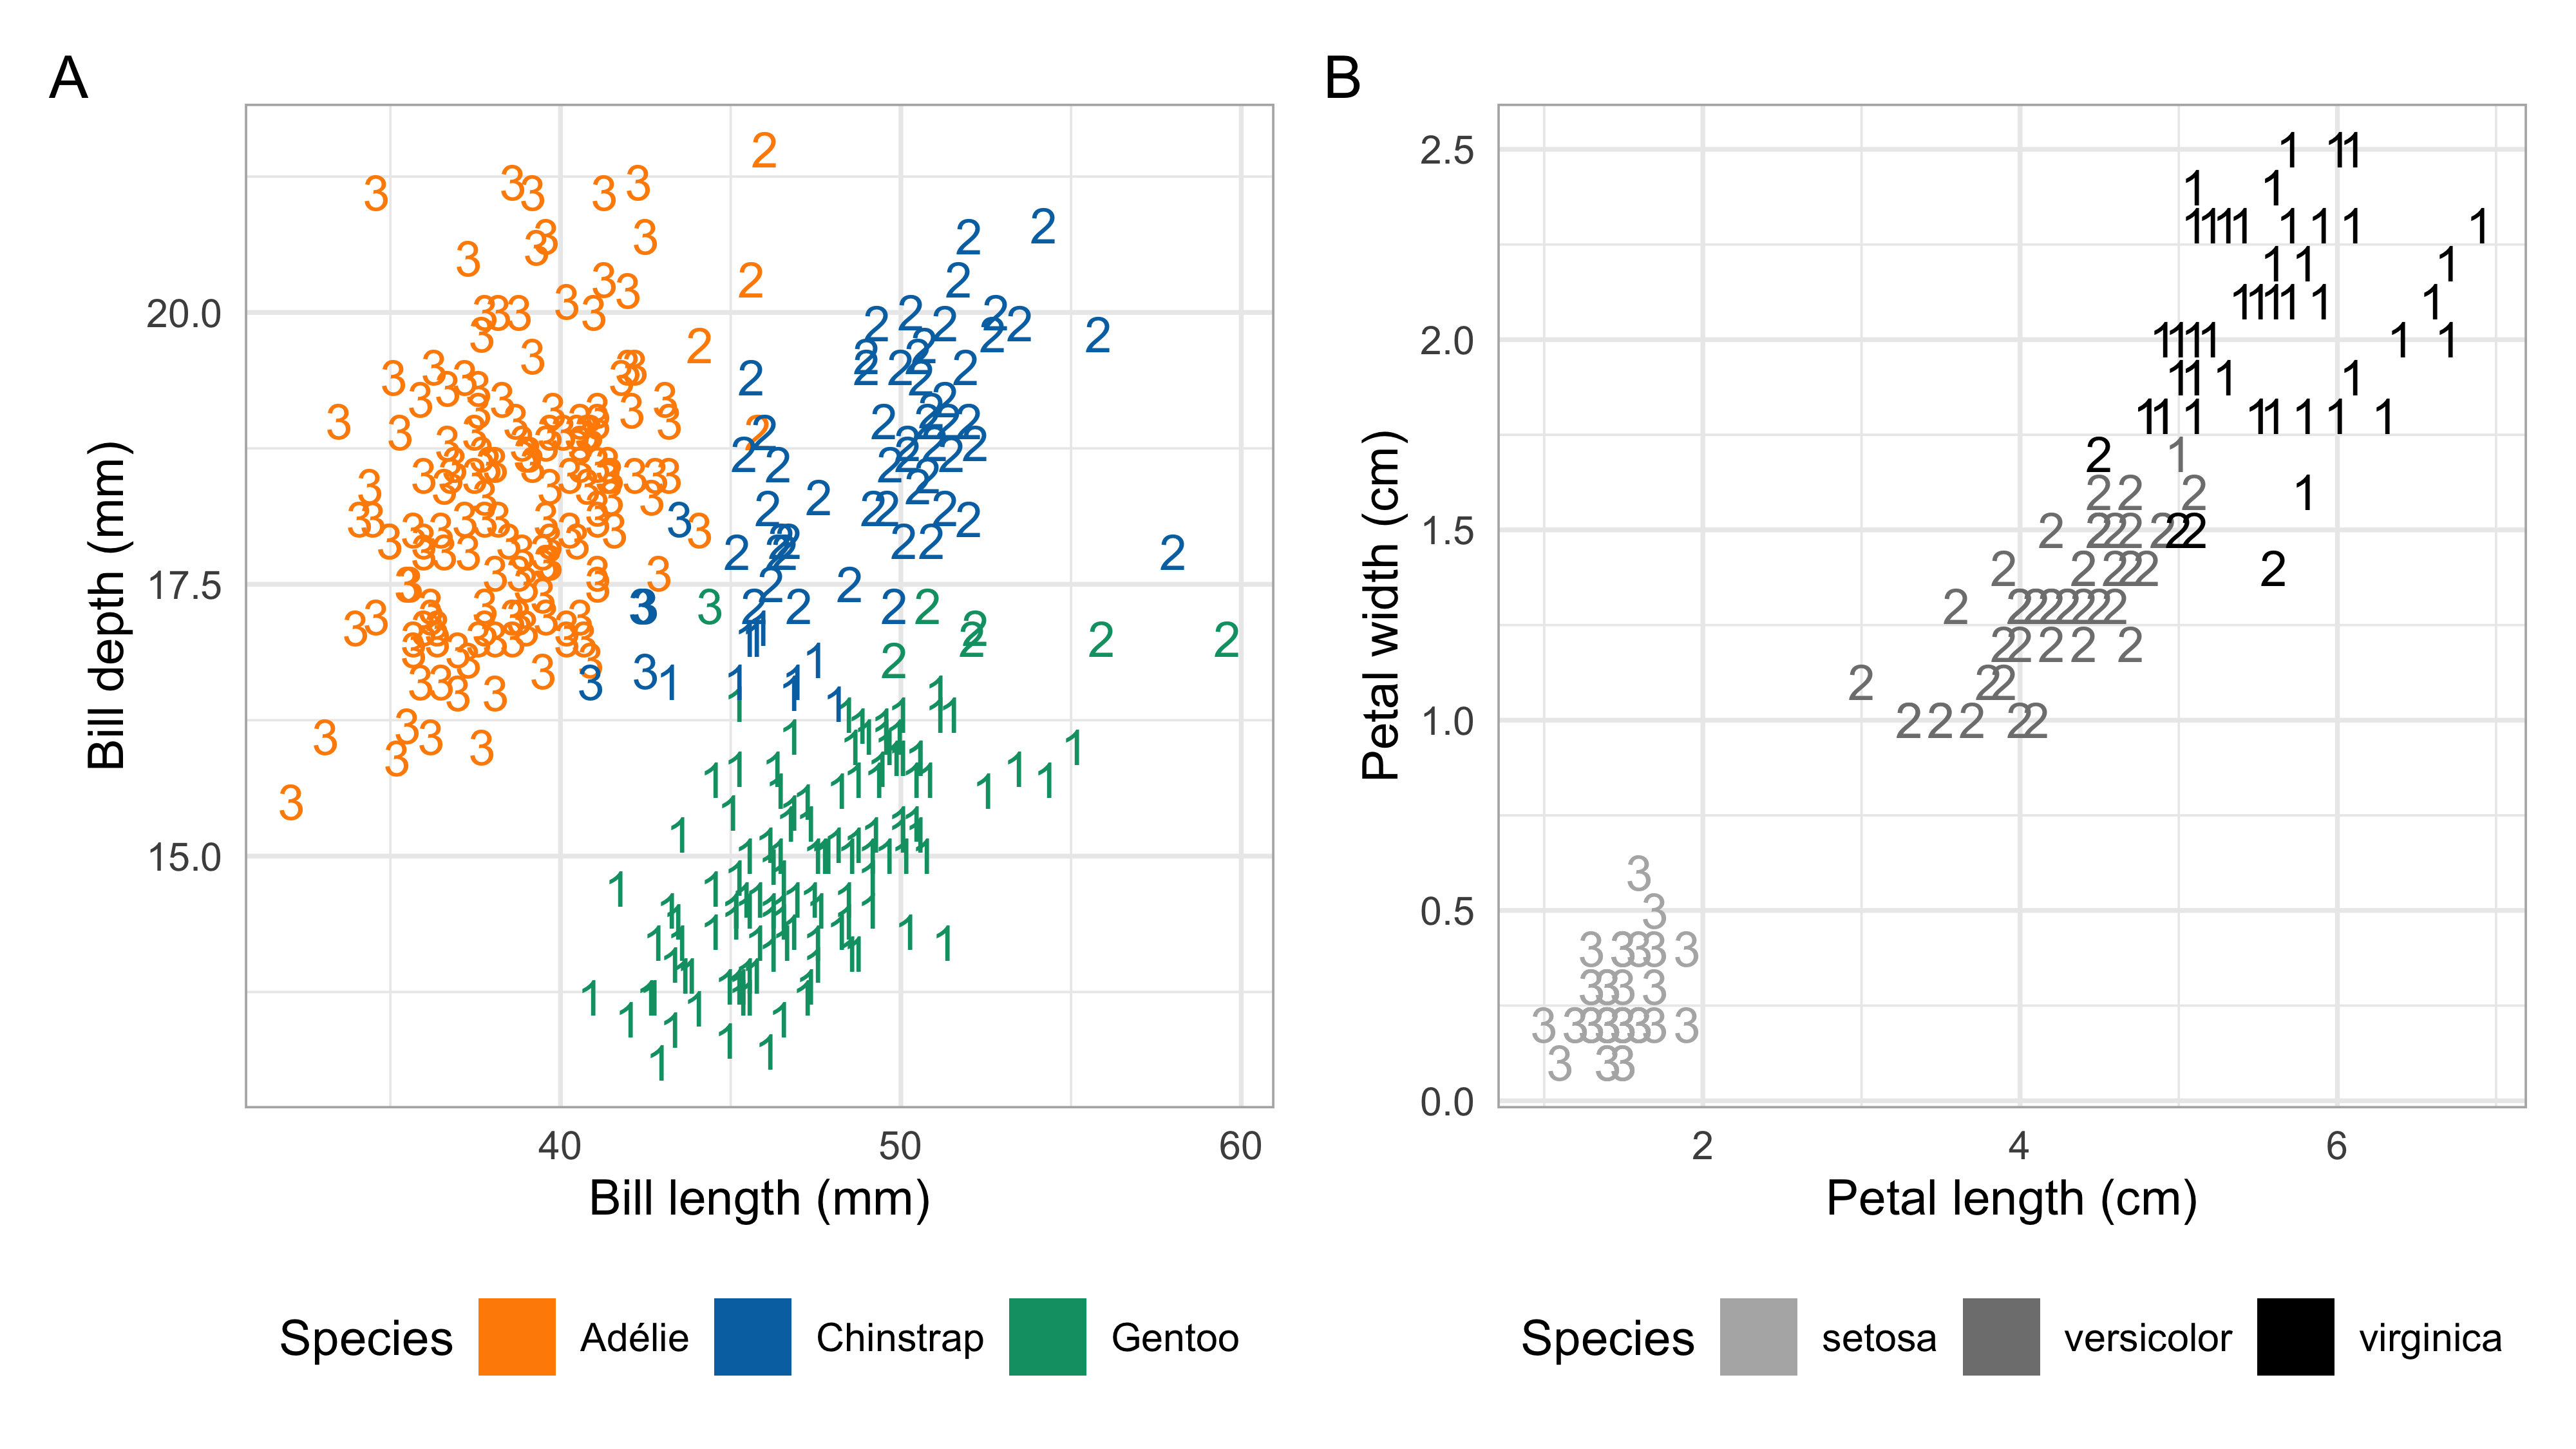
\includegraphics[width=6in]{fig/kmeans} 

}

\caption[K-means clustering outcomes for penguin bill dimensions (A) and iris petal dimensions (B)]{K-means clustering outcomes for penguin bill dimensions (A) and iris petal dimensions (B). Numbers indicate the cluster to which an observation was assigned, revealing a high degree of separation between species for both penguins and iris.}\label{fig:kmeans}
\end{figure}
\end{Schunk}

\begin{Schunk}
\begin{table}

\caption{\label{tab:unnamed-chunk-3}K-means cluster assignments by species based on penguin bill length (mm) and depth (mm), and iris petal length (cm) and width (cm).}
\centering
\begin{tabular}[t]{c|c|c|c|c|c|c|c}
\hline
\multicolumn{4}{c|}{Penguins cluster assignments} & \multicolumn{4}{c}{Iris cluster assignments} \\
\cline{1-4} \cline{5-8}
Cluster & Adélie & chinstrap & gentoo & Cluster & setosa & versicolor & virginica\\
\hline
1 & NA & 9 & 116 & 1 & NA & 48 & 4\\
\hline
2 & 4 & 54 & 6 & 2 & NA & 2 & 46\\
\hline
3 & 147 & 5 & 1 & 3 & 50 & NA & NA\\
\hline
\end{tabular}
\end{table}

\end{Schunk}

\hypertarget{other-alternatives-to-iris}{%
\subsection{Other alternatives to
iris}\label{other-alternatives-to-iris}}

\hypertarget{discussion}{%
\subsection{Discussion}\label{discussion}}

Educators have three options regarding \textbf{iris} use in course
materials:

\begin{enumerate}
\def\labelenumi{\arabic{enumi}.}
\tightlist
\item
  Use \textbf{iris} without addressing its use in Fisher's eugenics
  research
\item
  Use \textbf{iris} \emph{and} address its use in Fisher's eugenics
  research
\item
  Replace \textbf{iris} with an alternative dataset offering similar
  teaching and learning opportunities
\end{enumerate}

Here, we have shown that structural size measurements for Palmer
Archipelago \emph{Pygoscelis} penguins, available as \textbf{penguins}
in the \textbf{palmerpenguins} R package, can replace \textbf{iris} for
a number of common use cases in data science and statistics education
including exploratory data visualization, linear correlation and
regression, PCA, and clustering by k-means. In addition, teaching and
learning opportunities in \textbf{penguins} are increased due to a
greater number of variables, missing values, unequal sample sizes, and
Simpson's paradox examples.

The \textbf{iris} dataset is widespread today because it was employed by
Fisher to advance statistical methods for eugenics research. While the
\emph{Irises} were described in Anderson's 1935 article in \emph{The
Bulletin of the American Iris Society} \citep{anderson_irises_1935}, the
measurements were published in full in Fisher's 1936 \emph{Annals of
Eugenics} publication \citep{fisher_use_1936} - a journal for which
Fisher served as editor before becoming chair of the Department of
Eugenics at University College London.

\hypertarget{conclusion}{%
\subsection{Conclusion}\label{conclusion}}

\hypertarget{appendix}{%
\subsection{Appendix}\label{appendix}}

\hypertarget{appendix-a}{%
\subsubsection{Appendix A}\label{appendix-a}}

\hypertarget{appendix-b}{%
\subsubsection{Appendix B}\label{appendix-b}}

Data in the \textbf{penguins} object have been minimally updated from
\textbf{penguins\_raw} as follows:

\begin{itemize}
\tightlist
\item
  All variable names are converted to lower snake case
\item
  Entries in \emph{species} are truncated to only include the common
  name (e.g.~``gentoo'', instead of ``gentoo penguin (Pygoscelis
  papua)'')
\item
  Recorded sex for penguin N36A1, originally recorded as ``.'', is
  updated to \texttt{NA}
\item
  \emph{culmen\_length\_mm} and \emph{culmen\_depth\_mm} variable names
  are updated to \emph{bill\_length\_mm} and \emph{bill\_depth\_mm},
  respectively
\item
  Class for categorical variables (\emph{species}, \emph{island},
  \emph{sex}) is updated to factor
\item
  Variable \emph{year} was pulled from clutch observations
\end{itemize}

\bibliography{RJreferences}


\address{%
Allison M. Horst\\
Bren School of Environmental Science and Management\\
University of California, Santa Barbara\\ Santa Barbara, CA 93106-5131\\
}
\href{mailto:ahorst@ucsb.edu}{\nolinkurl{ahorst@ucsb.edu}}

\address{%
Alison P. Hill\\
RStudio, PBC\\
250 Northern Ave\\ Boston, MA 02210\\
}
\href{mailto:alison@rstudio.com}{\nolinkurl{alison@rstudio.com}}

\address{%
Kristen B. Gorman\\
University of Alaska Fairbanks College of Fisheries and Ocean Sciences\\
2150 Koyukuk Drive\\ 245 O'Neill Building\\ Fairbanks, AK 99775-7220\\
}
\href{mailto:kbgorman@alaska.edu}{\nolinkurl{kbgorman@alaska.edu}}

